\chapter{5G Mobile Networks: Beamforming, Random Access, and High-Capacity Protocols}
\label{sec:chapter4}

The fifth-generation (5G) New Radio (NR) cellular standard, developed by the Third Generation Partnership Project (3GPP) across Releases~15, 16, and 17, departs fundamentally from legacy cellular generations. While previous cellular architectures were primarily optimized for uniform wide-area enhanced Mobile Broadband (eMBB) human-centric traffic, 5G is designed as a multi-service wireless infrastructure supporting three radically divergent use cases:
\begin{enumerate}
    \item \textbf{Enhanced Mobile Broadband (eMBB):} Delivering gigabit-per-second peak user throughputs, extreme spectral efficiency, and high network capacity across dense urban topologies.
    \item \textbf{Ultra-Reliable Low-Latency Communication (URLLC):} Providing sub-millisecond radio access latencies with strict packet delivery reliability exceeding $99.999\%$ (five-nines) for mission-critical industrial automation, intelligent transportation systems, and tactile internet applications.
    \item \textbf{Massive Machine-Type Communications (mMTC):} Supporting hyper-dense deployments of up to $10^6$ low-cost, battery-constrained Internet of Things (IoT) sensors and actuators per square kilometre transmitting sporadic, bursty packets under constrained bandwidth.
\end{enumerate}

To simultaneously address these conflicting design goals, 5G NR spans an expansive spectrum portfolio partitioned into two distinct frequency regimes: Frequency Range~1 (FR1, sub-6~GHz, extending from $410\text{~MHz}$ to $7.125\text{~GHz}$) and Frequency Range~2 (FR2, millimeter-wave or mmWave, spanning $24.25\text{~GHz}$ to $52.6\text{~GHz}$ and beyond up to $71\text{~GHz}$). 

While mmWave spectrum offers immense contiguous bandwidths exceeding several hundreds of megahertz, high-frequency radio propagation suffers from severe free-space path loss, severe atmospheric oxygen and water vapor absorption, weak diffraction, and extreme sensitivity to physical obstacle blockage by buildings, human bodies, and foliage. Consequently, 5G base stations (next-generation NodeB or gNB) and user equipments (UEs) must deploy massive Multiple-Input Multiple-Output (massive MIMO) antenna arrays to synthesize highly directional narrow beams. The resulting array gain compensates for the steep path loss and establishes viable link budgets.

However, the transition from quasi-omnidirectional broadcast coverage to sharp directional beamforming introduces intricate cross-layer bottlenecks in the initial synchronization and medium access control (MAC) connection establishment procedures:
\begin{itemize}
    \item \textbf{Directional Initial Access Latency:} Because directional beams illuminate only a fraction of the angular sector at any instant, the gNB must execute continuous periodic beam sweeping. UEs contending for network access experience variable discovery latencies that depend on synchronization burst periodicities and beam migration dynamics.
    \item \textbf{Preamble Capacity Exhaustion in mMTC:} Traditional cellular random access relies on Zadoff-Chu (ZC) sequences. Under 3GPP specifications, only 64 preambles are allocated per cell or beam. In massive IoT scenarios with millions of contending devices, severe preamble collisions occur, resulting in synchronization failure, channel congestion, and battery depletion.
    \item \textbf{Severe Obstacle Blockage and Shadowing in mmWave:} At mmWave frequencies, even small physical obstacles abruptly sever Line-of-Sight (LoS) links, dropping received signal levels by 20 to 40~dB. When coupled with user mobility and spatial clustering of interferers, the random access channel (PRACH) experiences severe signal-to-interference-plus-noise ratio (SINR) degradation and outage.
\end{itemize}

This chapter synthesizes the foundational analytical and protocol contributions developed by Lokesh Bommisetty, Sagar Pawar, and T.~G.~Venkatesh \cite{pawar2023high, bommisetty2023connection, bommisetty2022mmwave, bommisetty2024contextual}. The sections develop rigorous mathematical frameworks for high-capacity preamble design, directional connection establishment queueing dynamics, stochastic blockage modeling via $M/G/\infty$ queueing analogies, and contextual bandit-based adaptive numerology.

---

\section{High-Capacity Preamble Sequence Design for 5G IoT Networks}
\label{sec:5g_preamble_design}

Random access is the foundational handshake protocol enabling an uncoordinated UE to establish uplink frame synchronization, request uplink shared channel grants, and transition from idle or inactive state to connected mode.

\subsection{Limitations of Legacy Zadoff-Chu Sequences}
In legacy 4G LTE and standard 5G NR specifications (3GPP TS 38.211), Physical Random Access Channel (PRACH) preambles are generated from Zadoff-Chu (ZC) sequences. A root ZC sequence $x_u[n]$ of prime length $L_{\mathrm{RA}}$ and root index $u \in \{1, 2, \dots, L_{\mathrm{RA}}-1\}$ is defined as:
\begin{equation}
    \label{eq:zc_definition}
    x_u[n] = \exp\left( -j \frac{\pi u n (n + 1)}{L_{\mathrm{RA}}} \right), \qquad 0 \le n \le L_{\mathrm{RA}} - 1
\end{equation}
where $\gcd(u, L_{\mathrm{RA}}) = 1$. ZC sequences exhibit the Constant Amplitude Zero Auto-Correlation (CAZAC) property:
\begin{enumerate}
    \item Ideal periodic auto-correlation:
    \begin{equation}
        R_{x_u, x_u}[d] = \sum_{n=0}^{L_{\mathrm{RA}}-1} x_u[n] x_u^*[(n+d) \bmod L_{\mathrm{RA}}] = L_{\mathrm{RA}} \cdot \delta[d]
    \end{equation}
    where $\delta[d]$ is the Kronecker delta function.
    \item Bounded cross-correlation: Between any two distinct roots $u_1 \ne u_2$, the periodic cross-correlation magnitude satisfies Welch's lower bound:
    \begin{equation}
        |R_{x_{u_1}, x_{u_2}}[d]| = \frac{1}{\sqrt{L_{\mathrm{RA}}}}, \qquad \forall d
    \end{equation}
\end{enumerate}

To generate multiple orthogonal preambles from a single root sequence $u$, cyclic shifts $C_v = v N_{\mathrm{CS}}$ are applied, where $N_{\mathrm{CS}}$ denotes the cyclic shift length configured by the network based on the maximum cell radius and channel delay spread:
\begin{equation}
    x_{u, v}[n] = x_u[(n + C_v) \bmod L_{\mathrm{RA}}]
\end{equation}
The cyclic shift step $N_{\mathrm{CS}}$ defines a Zero Correlation Zone (ZCZ) that prevents timing uncertainty and multipath delay spread from leaking into adjacent preamble detection bins. Consequently, the total number of preambles that can be derived from a single root sequence is bounded by $\lfloor L_{\mathrm{RA}} / N_{\mathrm{CS}} \rfloor$. The aggregate preamble capacity $C_{\mathrm{ZC}}$ across all $L_{\mathrm{RA}} - 1$ distinct roots is:
\begin{equation}
    \label{eq:zc_capacity}
    C_{\mathrm{ZC}} = (L_{\mathrm{RA}} - 1) \left\lfloor \frac{L_{\mathrm{RA}}}{N_{\mathrm{CS}}} \right\rfloor
\end{equation}

In standard 5G deployments, exactly 64 preambles are allocated per cell. When $N_{\mathrm{CS}}$ is configured to accommodate moderate cell radii (e.g., $N_{\mathrm{CS}} = 13$ for $L_{\mathrm{RA}} = 139$, or $N_{\mathrm{CS}} = 119$ for $L_{\mathrm{RA}} = 839$), only a tiny fraction of preambles can be formed per root, forcing the reuse of root preambles. In massive machine-type communications (mMTC) where tens of thousands of IoT sensors wake up simultaneously (e.g., following smart grid outages or environmental triggers), 64 preambles lead to devastating collision probabilities exceeding $50\%$.

While modified ZC (mZC) and augmented ZC (aZC) sequences were investigated in the literature, they introduce severe parameter ambiguities and phase coupling. Specifically, when modulating phase parameters $\lambda, w, \mu$, multiple parameter combinations produce identical correlation peaks, yielding high false-alarm rates and limiting the usable unambiguous sequence capacity to the order of $10^5$, which falls short of the $10^6\text{~devices/km}^2$ 5G mMTC density target \cite{pawar2023high}.

\subsection{Construction of Modified Alltop (mALL) Preamble Sequences}
To break the capacity bottleneck of CAZAC preambles, Pawar, Bommisetty, and Venkatesh \cite{pawar2023high} proposed a novel family of multi-parameter sequences termed \textbf{modified Alltop (mALL)} sequences.

The construction builds upon cubic phase Alltop sequences. For a sequence length $L_{\mathrm{RA}} \ge 5$ chosen as a prime number, an Alltop sequence $a_{\lambda, w}^{(l)}[n]$ governed by cubic index $l$, quadratic parameter $\lambda$, and linear parameter $w$ is defined as:
\begin{equation}
    \label{eq:alltop_def}
    a_{\lambda, w}^{(l)}[n] = \exp\left( j \frac{2\pi}{L_{\mathrm{RA}}} \left( l n^3 + \lambda n^2 + w n \right) \right), \qquad 0 \le l, \lambda, w, n \le L_{\mathrm{RA}} - 1
\end{equation}
For fixed $l$ and $\lambda$, varying the parameter $w$ generates a cyclic shifted replica of the sequence. Consequently, taking the periodic cross-correlation of two Alltop sequences with identical $(l, \lambda)$ but distinct $(w, w')$ yields an elevated cross-correlation peak, restricting the unambiguous family size to variations of $l$ and $\lambda$ only.

To decouple the correlation peak from the linear shift parameter $w$, Pawar et al. \cite{pawar2023high} introduced maximum length sequences ($m$-sequences) as multiplicative cover sequences. Let $x_m[n]$ represent an $m$-sequence of period $L_{\mathrm{RA}}$, and let $x_m^t[n] = x_m[(n + t) \bmod L_{\mathrm{RA}}]$ denote its $t$-th cyclic shift. The proposed **mALL preamble sequence** $z_{l, \lambda, w, t}[n]$ is synthesized as:
\begin{equation}
    \label{eq:mall_definition}
    z_{l, \lambda, w, t}[n] = a_{\lambda, w}^{(l)}[n] \odot x_m^t[n] = \exp\left( j \frac{2\pi}{L_{\mathrm{RA}}} \left( l n^3 + \lambda n^2 + w n \right) \right) \cdot x_m[(n + t) \bmod L_{\mathrm{RA}}]
\end{equation}
where $\odot$ denotes element-wise Hadamard multiplication, and $0 \le l, \lambda, w, t, n \le L_{\mathrm{RA}} - 1$.

Extensive periodic auto- and cross-correlation evaluations establish the following key properties of mALL sequences:
\begin{itemize}
    \item \textbf{Ideal Auto-Correlation:} For any parameter tuple $\{l, \lambda, w, t\}$, the auto-correlation exhibits a single delta peak of height $L_{\mathrm{RA}}$ at zero shift ($d = 0$), with all out-of-phase correlation values residing strictly within the low correlation zone (LCZ).
    \item \textbf{Bounded Cross-Correlation:} For arbitrary parameter tuples $\{l_1, \lambda_1, w_1\}$ and $\{l_2, \lambda_2, w_2\}$ with fixed cover parameter $t$, the average maximum cross-correlation magnitude is strictly bounded by:
    \begin{equation}
        \max_d |R_{z_1, z_2}[d]| < \sqrt{3 L_{\mathrm{RA}}}
    \end{equation}
    For $L_{\mathrm{RA}} = 139$, $\sqrt{3 L_{\mathrm{RA}}} \approx 20.42$, and the observed empirical mean maximum cross-correlation peak is $27.37$, which remains well below detection decision thresholds.
    \item \textbf{Unambiguous Family Selection:} While allowing $t$ to vary concurrently with $(l, \lambda, w)$ introduces rare correlation ambiguities, holding $t$ constant (e.g., $t = 1$) across the cell yields a completely unambiguous, mutually quasi-orthogonal family across all permutations of $(l, \lambda, w)$.
\end{itemize}

\subsection{Aggregate Preamble Capacity Expansion}
To further expand the capacity of available preambles within each cell, each generated sequence $z_{l, \lambda, w, t}[n]$ is cyclically shifted by integer multiples of $N_{\mathrm{CS}}$ according to the 3GPP zero correlation zone configuration:
\begin{equation}
    z_{v, l, \lambda, w, t}[n] = z_{l, \lambda, w, t}[(n + C_v) \bmod L_{\mathrm{RA}}], \qquad C_v = v N_{\mathrm{CS}}, \quad v \in \left\{ 0, 1, \dots, \left\lfloor \frac{L_{\mathrm{RA}}}{N_{\mathrm{CS}}} \right\rfloor - 1 \right\}
\end{equation}

Let $\mathcal{S}_v^{\mathrm{mALL}} = \bigcup_{l, \lambda, w} \{ z_{v, l, \lambda, w, t}[n] \}$ represent the set of all non-ambiguous sequences for a given shift index $v$ under fixed $t$. Because $l, \lambda, w \in \{0, 1, \dots, L_{\mathrm{RA}}-1\}$, exactly $L_{\mathrm{RA}}^3$ unique sequences exist for each cyclic shift $v$. Taking the union across all permissible cyclic shifts yields the complete ensemble:
\begin{equation}
    \mathcal{S}^{\mathrm{mALL}} = \bigcup_{v=0}^{\lfloor L_{\mathrm{RA}}/N_{\mathrm{CS}} \rfloor - 1} \mathcal{S}_v^{\mathrm{mALL}}
\end{equation}
The total PRACH preamble capacity for the proposed mALL sequence family is therefore derived as \cite{pawar2023high}:
\begin{equation}
    \label{eq:mall_capacity}
    C_{\mathrm{mALL}} = L_{\mathrm{RA}} \times L_{\mathrm{RA}} \times L_{\mathrm{RA}} \times \left\lfloor \frac{L_{\mathrm{RA}}}{N_{\mathrm{CS}}} \right\rfloor = L_{\mathrm{RA}}^3 \left\lfloor \frac{L_{\mathrm{RA}}}{N_{\mathrm{CS}}} \right\rfloor
\end{equation}

\begin{table}[htbp]
\centering
\caption{Comparison of Preamble Capacity across Sequence Families ($L_{\mathrm{RA}} = 139$)}
\label{tab:preamble_capacity_comp}
\begin{tabular}{lcccc}
\toprule
\textbf{Preamble Family} & \textbf{Sequence Formulation} & $N_{\mathrm{CS}} = 13$ & $N_{\mathrm{CS}} = 7$ & $N_{\mathrm{CS}} = 2$ \\
\midrule
Legacy Zadoff-Chu (ZC) \cite{3gpp38211} & Quadratic Phase & $1.38 \times 10^3$ & $2.62 \times 10^3$ & $9.52 \times 10^3$ \\
Modified ZC (mZC) \cite{pawar2023high} & Quadratic + Affine Phase & $1.92 \times 10^5$ & $3.64 \times 10^5$ & $1.32 \times 10^6$ \\
Augmented ZC (aZC) & Cubic + Affine Phase & $1.92 \times 10^5$ & $3.64 \times 10^5$ & $1.32 \times 10^6$ \\
\textbf{Proposed mALL} \cite{pawar2023high} & \textbf{Cubic Alltop $\odot$ $m$-sequence} & $\mathbf{2.68 \times 10^7}$ & $\mathbf{5.10 \times 10^7}$ & $\mathbf{1.85 \times 10^8}$ \\
\bottomrule
\end{tabular}
\end{table}

As documented in Table~\ref{tab:preamble_capacity_comp}, for $L_{\mathrm{RA}} = 139$ and $N_{\mathrm{CS}} = 13$, the legacy ZC sequence yields only $1{,}380$ candidate preambles cell-wide, from which 64 must be partitioned. In stark contrast, the proposed mALL sequence delivers over $2.68 \times 10^7$ unique preambles. This represents a four-orders-of-magnitude ($> 19{,}000\times$) capacity expansion over ZC sequences. This massive capacity headroom allows base stations to allocate unique preambles to individual IoT devices or small device clusters, virtually eliminating random access preamble collisions in hyper-dense mMTC deployments.

\subsection{Receiver Architecture and Constant False-Alarm Rate (CFAR) Detection}
To detect contending preambles without prohibitive receiver complexity, Pawar et al. \cite{pawar2023high} developed an efficient frequency-domain detection pipeline exploiting multi-antenna diversity combining and adaptive thresholding.

\begin{figure}[htbp]
    \centering
    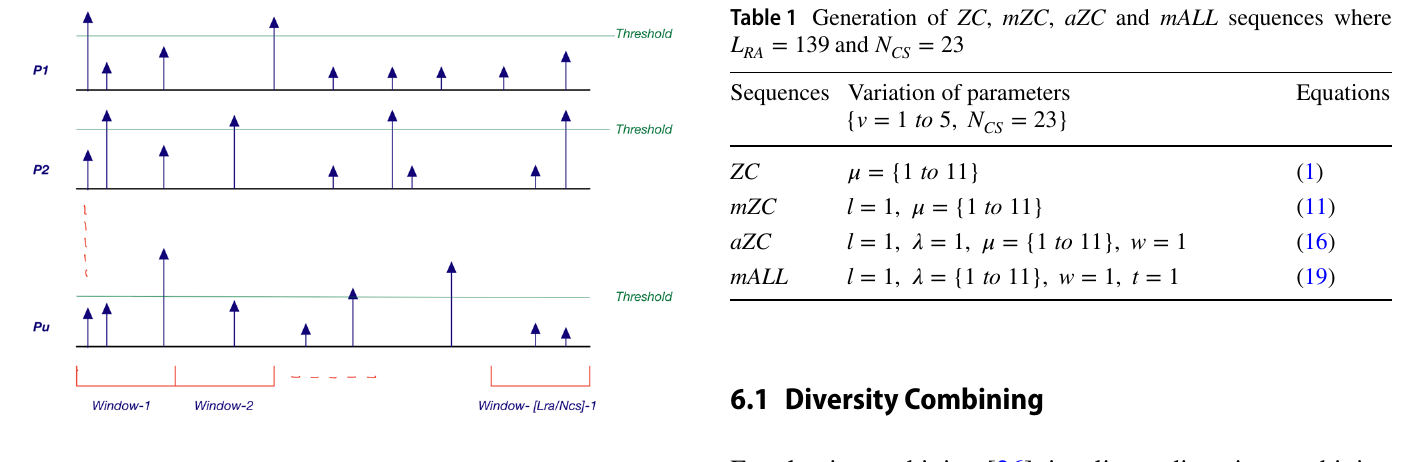
\includegraphics[width=0.75\textwidth]{figures/fig_5g_pdp_detection.png}
    \caption{Multi-antenna Power Delay Profile (PDP) accumulation and CFAR threshold preamble detection algorithm \cite{pawar2023high}.}
    \label{fig:5g_pdp_detection}
\end{figure}

The receiver processing workflow illustrated in Figure~\ref{fig:5g_pdp_detection} proceeds as follows:
\begin{enumerate}
    \item \textbf{Equal Gain Combining (EGC):} Let $N_{\mathrm{Ant}}$ denote the number of receive antenna branches at the gNB. Let $s_i[n]$ represent the time-domain received baseband signal at antenna $i \in \{1, \dots, N_{\mathrm{Ant}}\}$, and let $k_\mu[n]$ denote the candidate root sequence available at the receiver. Using the Discrete Fourier Transform (DFT), circular cross-correlation matrix $\mathbf{R}_{s_i, k_\mu}$ is computed efficiently via element-wise multiplication in the frequency domain:
    \begin{equation}
        R_{s_i, k_\mu}[d] = \mathrm{IDFT}\left\{ \mathrm{DFT}\{s_i[n]\} \cdot \left(\mathrm{DFT}\{k_\mu[n]\}\right)^* \right\}
    \end{equation}
    \item \textbf{Power Delay Profile (PDP) Accumulation:} The instantaneous PDP matrix $\mathbf{P}_{i, \mu}$ for antenna branch $i$ is formed by taking the squared magnitude of correlation entries:
    \begin{equation}
        P_{i, \mu}[d] = |R_{s_i, k_\mu}[d]|^2, \qquad 0 \le d \le L_{\mathrm{RA}} - 1
    \end{equation}
    The diversity PDP across all $N_{\mathrm{Ant}}$ antennas is accumulated via Equal Gain Combining:
    \begin{equation}
        \label{eq:egc_pdp}
        P_\mu^{N_{\mathrm{Ant}}}[d] = \sum_{i=1}^{N_{\mathrm{Ant}}} P_{i, \mu}[d] = \sum_{i=1}^{N_{\mathrm{Ant}}} |R_{s_i, k_\mu}[d]|^2
    \end{equation}
    \item \textbf{Window Partitioning and Normalization:} Each row of the accumulated PDP is partitioned into $W = \lfloor L_{\mathrm{RA}} / N_{\mathrm{CS}} \rfloor$ non-overlapping detection windows of length $N_{\mathrm{CS}}$. The baseline noise power level is estimated by the mean of the accumulated profile:
    \begin{equation}
        \bar{P}_\mu^{N_{\mathrm{Ant}}} = \frac{1}{L_{\mathrm{RA}}} \sum_{d=0}^{L_{\mathrm{RA}}-1} P_\mu^{N_{\mathrm{Ant}}}[d]
    \end{equation}
    The normalized detection profile is:
    \begin{equation}
        P_{\mu, \mathrm{norm}}^{N_{\mathrm{Ant}}}[d] = \frac{P_\mu^{N_{\mathrm{Ant}}}[d]}{\bar{P}_\mu^{N_{\mathrm{Ant}}}}
    \end{equation}
    \item \textbf{CFAR Peak Comparison:} A detection threshold $\eta$ is calibrated to satisfy the strict 3GPP requirement that the false alarm probability does not exceed $0.1\%$ ($P_{\mathrm{false}} \le 10^{-3}$):
    \begin{equation}
        P_{\mathrm{false}} = \mathbb{P}\left( \max_{d \in \mathrm{window}} P_{\mu, \mathrm{norm}}^{N_{\mathrm{Ant}}}[d] > \eta \;\Bigg|\; \text{No preamble transmitted} \right) \le 0.001
    \end{equation}
    If the peak normalized correlation in any window exceeds $\eta$, a preamble transmission is declared, and the delay location of the peak provides the timing advance estimate $\hat{\tau}_{\mathrm{TA}}$.
\end{enumerate}

Simulations under additive white Gaussian noise (AWGN) and multipath Rayleigh fading channels demonstrate that mALL sequences achieve $99\%$ detection probability ($P_{\mathrm{det}} \ge 0.99$) at an SNR of $-6.5\text{~dB}$ in a $1\text{-TX}, 1\text{-RX}$ antenna configuration, trailing the legacy ZC sequence by merely $0.3\text{~dB}$. With $N_{\mathrm{Ant}} = 2$ diversity combining, $P_{\mathrm{det}} \ge 0.99$ is achieved at $-10.2\text{~dB}$ \cite{pawar2023high}.

\subsection{Peak-to-Average Power Ratio (PAPR) and Cubic Metric}
Because preambles are transmitted on the uplink by battery-operated IoT transceivers, low envelope fluctuation is vital to avoid non-linear power amplifier distortion and battery drain. 

The Peak-to-Average Power Ratio (PAPR) of the time-domain signal $s(t)$ over duration $T$ is defined as:
\begin{equation}
    \mathrm{PAPR} = \frac{\max_{0 \le t \le T} |s(t)|^2}{\frac{1}{T} \int_0^T |s(t)|^2 dt}
\end{equation}
Complementary Cumulative Distribution Function (CCDF) evaluations show that at the $99\%$ point ($\mathrm{CCDF} = 10^{-2}$), the PAPR of the proposed mALL sequence is $7.1\text{~dB}$, which is comparable to mZC ($7.4\text{~dB}$) and legacy ZC ($7.2\text{~dB}$). Furthermore, the 3GPP Cubic Metric (CM), which directly quantifies required power amplifier backoff, is measured at $1.52\text{~dB}$ for mALL, matching that of legacy ZC sequences \cite{pawar2023high}. Thus, mALL sequences achieve four orders of magnitude higher preamble capacity with zero penalty in RF amplifier efficiency.

---

\section{5G NR Connection Establishment Under Directional Beamforming}
\label{sec:5g_connection_beamforming}

At high frequencies in FR1 and mmWave bands in FR2, isotropic coverage is impossible due to severe path loss. The 5G NR physical layer consequently relies on directional beam sweeping during cell search and random access. Bommisetty and Venkatesh \cite{bommisetty2023connection} formulated the first comprehensive queueing analytical framework capturing the interaction between directional beam sweeping, preamble contention, and association rules.

\subsection{Synchronization Signal Block (SSB) and SS Burst Architecture}
Initial synchronization and system acquisition in 5G NR revolve around the \textbf{Synchronization Signal Block (SSB)}, structured across time and frequency as depicted in Figure~\ref{fig:5g_ssb_structure}.

\begin{figure}[htbp]
    \centering
    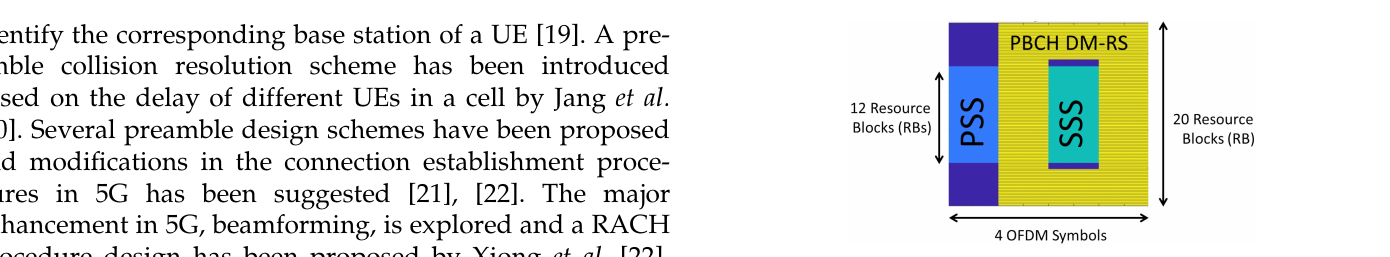
\includegraphics[width=0.75\textwidth]{figures/fig_5g_ssb_structure.png}
    \caption{Time-frequency frame structure of a 5G NR Synchronization Signal Block (SSB) across 4 OFDM symbols and 240 subcarriers \cite{bommisetty2023connection}.}
    \label{fig:5g_ssb_structure}
\end{figure}

An SSB spans exactly 4 OFDM symbols in the time domain and 240 contiguous subcarriers (corresponding to 20 Resource Blocks) in the frequency domain:
\begin{itemize}
    \item \textbf{Primary Synchronization Signal (PSS):} Occupies Symbol~0, spanning 127 subcarriers centered within the 240-subcarrier block (subcarriers 56 to 182). Formed from frequency-domain $m$-sequences, it conveys the physical layer cell sub-identity $N_{\mathrm{ID}}^{(2)} \in \{0, 1, 2\}$.
    \item \textbf{Secondary Synchronization Signal (SSS):} Occupies Symbol~2, spanning 127 subcarriers. It conveys the cell group identity $N_{\mathrm{ID}}^{(1)} \in \{0, 1, \dots, 335\}$, establishing the complete Physical Cell ID (PCI): $N_{\mathrm{ID}}^{\mathrm{cell}} = 3 N_{\mathrm{ID}}^{(1)} + N_{\mathrm{ID}}^{(2)}$.
    \item \textbf{Physical Broadcast Channel (PBCH):} Spans Symbol~1, Symbol~3, and the subcarriers flanking the SSS in Symbol~2 (48 subcarriers on either side). The PBCH carries the Master Information Block (MIB), Demodulation Reference Signals (DMRS) for coherent channel estimation, and timing parameters for decoding System Information Block~1 (SIB1).
\end{itemize}

To illuminate the entire cell sector, multiple SSBs are transmitted in distinct spatial directions via beam sweeping, forming an \textbf{SS Burst}. All SSBs constituting an SS Burst must be transmitted within a $5\text{~ms}$ half-frame window. The maximum number of SSBs in a burst, denoted by $L_{\max}$, scales with the operational frequency carrier:
\begin{equation}
    L_{\max} = \begin{cases}
        4, & f_c < 3\text{~GHz} \\
        8, & 3\text{~GHz} \le f_c \le 6\text{~GHz} \\
        64, & f_c > 6\text{~GHz (mmWave FR2)}
    \end{cases}
\end{equation}
The nominal periodicity of SS Burst sweeping is configured by the network parameter $T_{\mathrm{SSB}}$, defaulting to $20\text{~ms}$ (2 frames) for initial cell search.

\subsection{Random Access Procedure and SSB-to-PRACH Occasion Mapping}
Following successful SSB acquisition and MIB/SIB1 decoding, the UE identifies the optimal downlink beam (SSB index) based on maximum Reference Signal Received Power (RSRP). To initiate connection establishment, the UE must transmit a PRACH preamble in an uplink beam oriented toward the gNB.

\begin{figure}[htbp]
    \centering
    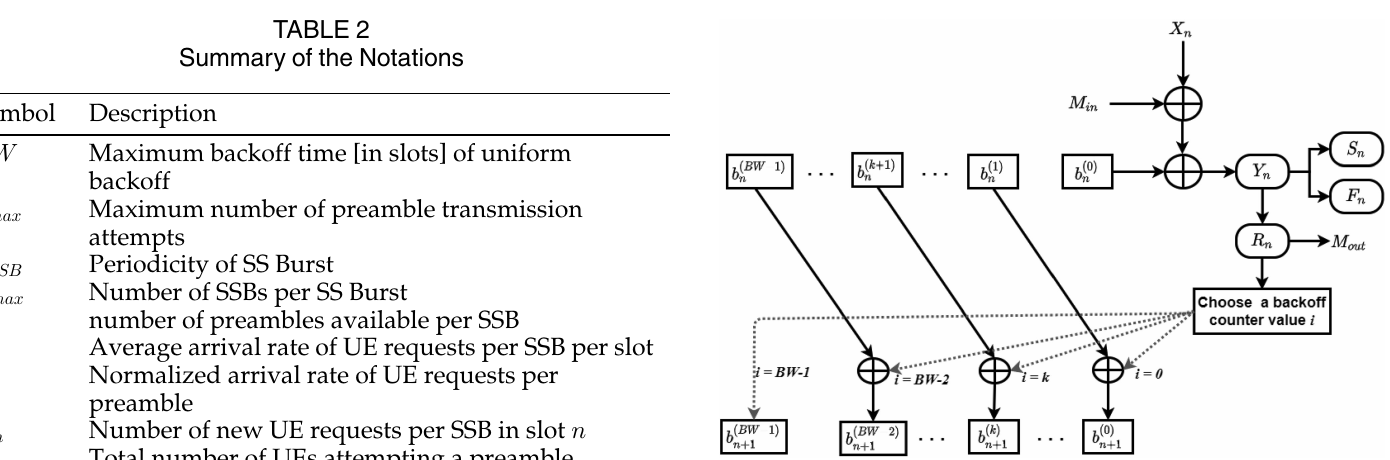
\includegraphics[width=0.85\textwidth]{figures/fig_5g_connection_model.png}
    \caption{Queueing and connection establishment system model under directional beam sweeping and beam migration \cite{bommisetty2023connection}.}
    \label{fig:5g_connection_model}
\end{figure}

The relationship between downlink SSBs and uplink PRACH Occasions (ROs) is governed by the 3GPP configuration parameter \texttt{ssb-perRACH-OccasionAndCB-PreamblesPerSSB}:
\begin{itemize}
    \item $N$: The number of distinct SSBs mapped to each PRACH occasion (e.g., $N \in \{1/8, 1/4, 1/2, 1, 2, 4, 8, 16\}$).
    \item $R$: The number of contention-based preambles assigned per SSB within that RO.
\end{itemize}

When $N$ SSBs share a single RO, the total pool of 64 preambles in that RO is subdivided into $N$ contiguous subsets, each containing $R$ preambles ($N \cdot R \le 64$). A UE synchronized to a specific SSB selects a preamble uniformly at random from its designated $R$-preamble subset.

The total duration required to map all $L_{\max}$ SSBs to corresponding ROs defines the \textbf{association period} $T_a$:
\begin{equation}
    \label{eq:association_period}
    T_a = \left\lceil \frac{L_{\max}}{N \cdot N_{\mathrm{RO}}^{\mathrm{slot}} \cdot N_{\mathrm{slot}}^{\mathrm{frame}}} \right\rceil T_p
\end{equation}
where $N_{\mathrm{RO}}^{\mathrm{slot}}$ is the number of time/frequency ROs per PRACH slot, $N_{\mathrm{slot}}^{\mathrm{frame}}$ is the number of PRACH slots per frame, and $T_p$ is the PRACH frame configuration periodicity (e.g., $20\text{~ms}$).

\subsection{Queueing System Model and Equilibrium Analysis}
To quantify contention dynamics under beam sweeping, Bommisetty and Venkatesh \cite{bommisetty2023connection} developed a discrete-time queueing model formulated on a tagged SSB beam. As shown in Figure~\ref{fig:5g_connection_model}, in any arbitrary PRACH slot $n$, UE requests transition between states:
\begin{enumerate}
    \item \textbf{New Arrivals ($X_n$):} New connection requests arrive within the coverage footprint of the tagged SSB according to an independent Poisson process with mean $\lambda$ requests per slot: $\mathbb{E}[X_n] = \lambda$.
    \item \textbf{Beam Migration ($M_n^{\mathrm{in}}, M_n^{\mathrm{out}}$):} Due to terminal mobility and dynamic channel blockage, UEs may lose beam alignment with their serving SSB and migrate to adjacent beams. Let $u_{u, b}$ denote the probability that UE $u$ does not migrate away from beam $b$ during an association interval. The beam transition probability matrix $\mathbf{Q}_u \in \mathbb{R}^{L_{\max} \times L_{\max}}$ is governed by:
    \begin{equation}
        [\mathbf{Q}_u]_{b, b'} = p_{b, b'} (1 - u_{u, b}), \qquad b \ne b'
    \end{equation}
    Assuming spatial uniformity of Poisson arrivals across cell sectors, the expected number of migrating arrivals balances the departures: $\mathbb{E}[M_n^{\mathrm{in}}] = \mathbb{E}[M_n^{\mathrm{out}}]$.
    \item \textbf{Departures ($S_n, F_n$):} Departures occur either when a UE successfully completes preamble transmission ($S_n$) or when a UE exhausts its maximum permitted retransmission limit $T_{\max}$ and is dropped from the network ($F_n$).
\end{enumerate}

Under steady-state stochastic equilibrium, the arrival and departure flows must balance:
\begin{equation}
    \label{eq:5g_equilibrium_balance}
    \mathbb{E}[X_n] = \mathbb{E}[S_n] + \mathbb{E}[F_n]
\end{equation}

Let $Y_n$ denote the total number of contending UEs (newly arriving plus backlogged retransmitting UEs) attempting preamble transmission in slot $n$. In steady state, $Y_n$ is Poisson distributed with mean $y = \mathbb{E}[Y_n]$. Because each contending UE selects one of the $R$ preambles with equal probability $1/R$, the channel behaves as a multi-channel slotted ALOHA system. The expected number of successful preambles per slot is derived as:
\begin{equation}
    \label{eq:expected_successes}
    \mathbb{E}[S_n] = y e^{-y/R}
\end{equation}
The steady-state success probability $f$ of any individual UE attempt in a slot is:
\begin{equation}
    \label{eq:f_def}
    f = \frac{\mathbb{E}[S_n]}{y} = e^{-y/R} \implies y = -R \ln f
\end{equation}
Substituting $y$ back into Equation~\eqref{eq:expected_successes} expresses expected successes directly as:
\begin{equation}
    \label{eq:Sn_f}
    \mathbb{E}[S_n] = -R f \ln f
\end{equation}

A connection request is definitively dropped if it suffers collisions across all $T_{\max}$ successive transmission attempts. Since collision events across retransmissions separated by randomized backoff are asymptotically independent, the drop probability $d$ is:
\begin{equation}
    \label{eq:drop_prob}
    d = (1 - f)^{T_{\max}}
\end{equation}
The expected number of dropped connection requests per slot is therefore:
\begin{equation}
    \label{eq:Fn_f}
    \mathbb{E}[F_n] = \mathbb{E}[X_n] \cdot d = \lambda (1 - f)^{T_{\max}}
\end{equation}

Substituting Equations~\eqref{eq:Sn_f} and \eqref{eq:Fn_f} into the flow balance Equation~\eqref{eq:5g_equilibrium_balance} yields:
\begin{equation}
    \lambda = -R f \ln f + \lambda (1 - f)^{T_{\max}}
\end{equation}
Dividing by $R$ and defining the normalized arrival rate per preamble as $r \triangleq \lambda / R$, we obtain the fundamental fixed-point equilibrium relationship \cite{bommisetty2023connection}:
\begin{equation}
    \label{eq:fixed_point_master}
    \frac{f}{r} = g(f) \triangleq \frac{(1 - f)^{T_{\max}} - 1}{\ln f}
\end{equation}

\subsection{Fixed-Point Bifurcation, Stability Regimes, and Inflection Points}
Equation~\eqref{eq:fixed_point_master} is highly non-linear with no closed-form algebraic inverse. In Figure~\ref{eq:fixed_point_master}, the left-hand side $f/r$ represents a ray through the origin with slope $1/r$, while the right-hand side $g(f)$ is a non-linear characteristic curve parameterized solely by $T_{\max}$.

\begin{figure}[htbp]
\centering
\begin{minipage}{0.48\textwidth}
    \centering
    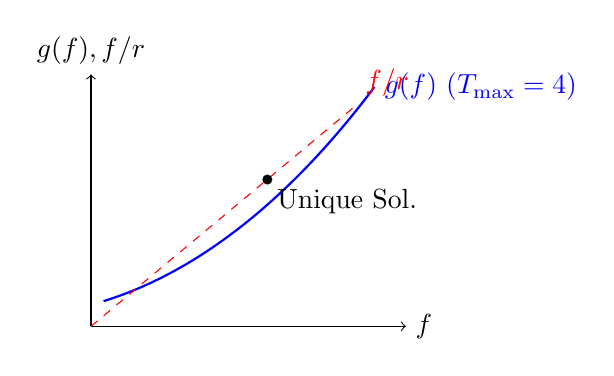
\begin{tikzpicture}[scale=0.8]
        \draw[->] (0,0) -- (5,0) node[right] {$f$};
        \draw[->] (0,0) -- (0,4) node[above] {$g(f), f/r$};
        \draw[thick, blue] (0.2, 0.4) .. controls (1.5, 0.8) and (3.0, 1.8) .. (4.5, 3.8) node[right] {$g(f)$ ($T_{\max}=4$)};
        \draw[dashed, red] (0,0) -- (4.2, 3.5) node[above right] {$f/r$};
        \filldraw[black] (2.8, 2.33) circle (2pt) node[below right] {Unique Sol.};
    \end{tikzpicture}
    \caption*{(a) Monostable Regime ($T_{\max} < 9$)}
\end{minipage}
\hfill
\begin{minipage}{0.48\textwidth}
    \centering
    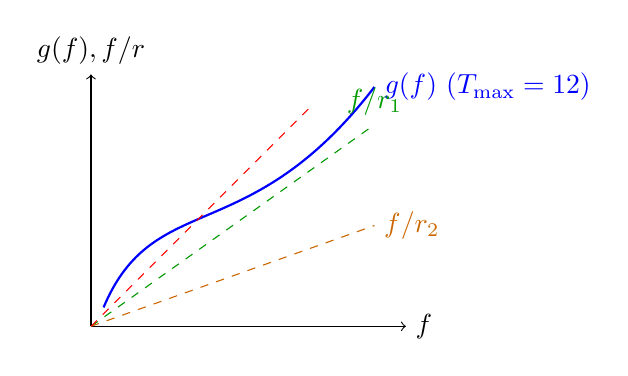
\begin{tikzpicture}[scale=0.8]
        \draw[->] (0,0) -- (5,0) node[right] {$f$};
        \draw[->] (0,0) -- (0,4) node[above] {$g(f), f/r$};
        \draw[thick, blue] (0.2, 0.3) .. controls (1.0, 2.2) and (2.5, 1.2) .. (4.5, 3.8) node[right] {$g(f)$ ($T_{\max}=12$)};
        \draw[dashed, green!60!black] (0,0) -- (4.5, 3.2) node[above] {$f/r_1$};
        \draw[dashed, orange!80!black] (0,0) -- (4.5, 1.6) node[right] {$f/r_2$};
        \draw[dashed, red] (0,0) -- (3.5, 3.5);
    \end{tikzpicture}
    \caption*{(b) Bistable / Hysteresis Regime ($T_{\max} \ge 9$)}
\end{minipage}
\caption{Fixed-point graphical solutions of $f/r = g(f)$ revealing stability bifurcation as a function of retransmission limit $T_{\max}$ \cite{bommisetty2023connection}.}
\label{fig:fixed_point_bifurcation}
\end{figure}

The analytical properties of $g(f)$ establish two fundamentally distinct operational regimes:
\begin{enumerate}
    \item \textbf{Monostable Regime ($T_{\max} < 9$):} For $T_{\max} \in \{1, 2, \dots, 8\}$, $g(f)$ is strictly increasing, convex, and differentiable throughout $f \in (0, 1)$. Consequently, the straight line $f/r$ intersects $g(f)$ at exactly one unique point for every positive arrival rate $r$. The system operates stably, and the success probability $f$ degrades smoothly and predictably with increasing traffic load $r$.
    \item \textbf{Bistable and Hysteresis Regime ($T_{\max} \ge 9$):} When $T_{\max} \ge 9$, $g(f)$ exhibits an inflection point, becoming piecewise concave and piecewise convex. Two distinct tangent lines crossing the origin can be drawn to $g(f)$, defined by tangent slopes $1/r_1$ and $1/r_2$ where $g'(f) = g(f)/f$:
    \begin{equation}
        \label{eq:tangent_boundaries}
        g'(f) = \frac{1}{r} \implies \frac{d}{df}\left[ \frac{(1 - f)^{T_{\max}} - 1}{\ln f} \right] = \frac{g(f)}{f}
    \end{equation}
    The tangent boundaries $(r_1, r_2)$ partition the network operating space into three regions:
    \begin{itemize}
        \item \textbf{Light-Load Stable Region ($r < r_1$):} A single high-throughput equilibrium point exists with high success probability $f$.
        \item \textbf{Bistable Hysteresis Region ($r_1 \le r \le r_2$):} Three equilibrium solutions appear (two stable roots flanking an unstable intermediate saddle point). Sudden transitions occur between high-success and congested states, generating severe jitter.
        \item \textbf{Congested Saturated Region ($r > r_2$):} The system collapses into a low-success, high-drop equilibrium where virtually all attempts fail ($d \to 1$).
    \end{itemize}
\end{enumerate}

Representative bifurcation threshold values computed by Bommisetty and Venkatesh \cite{bommisetty2023connection} are summarized in Table~\ref{tab:load_boundaries}.

\begin{table}[htbp]
\centering
\caption{Load Boundaries $r_1$ and $r_2$ for Transmission Attempt Limits $T_{\max}$ \cite{bommisetty2023connection}}
\label{tab:load_boundaries}
\begin{tabular}{cccc}
\toprule
\textbf{Boundary Parameter} & $T_{\max} = 12$ & $T_{\max} = 16$ & $T_{\max} = 20$ \\
\midrule
$r_1$ (Upper limit of low-load stability) & $0.305$ & $0.257$ & $0.215$ \\
$r_2$ (Lower limit of congested collapse) & $0.375$ & $0.375$ & $0.375$ \\
\bottomrule
\end{tabular}
\end{table}

\subsection{Performance Metrics: Joining Rate and Joining Latency Moments}
With equilibrium success probability $f$ resolved from Equation~\eqref{eq:fixed_point_master}, the primary network performance indicators are evaluated analytically:

\subsubsection{Average Joining Rate}
The average joining rate $J_{\mathrm{SSB}}$ represents the throughput of successful UEs entering the network per slot per SSB:
\begin{equation}
    \label{eq:joining_rate_ssb}
    J_{\mathrm{SSB}} = \lambda (1 - d) = \lambda \left[ 1 - (1 - f)^{T_{\max}} \right]
\end{equation}
At low arrival rates ($\lambda \to 0$), contention is negligible ($f \approx 1, d \approx 0$), yielding $J_{\mathrm{SSB}} \approx \lambda$. As arrival rate increases, $J_{\mathrm{SSB}}$ peaks at an optimal arrival rate $\lambda^* = r^* R$ (where $r^* \approx 0.4375$ for $T_{\max} = 4$), beyond which preamble collisions cause $d \to 1$ and $J_{\mathrm{SSB}}$ plummets to zero.

Scaling to the entire cell requires accounting for the association parameter $N$ and active SSBs $L_{\max}$. The cell-wide aggregate joining rate $J_{\mathrm{cell}}$ is:
\begin{equation}
    \label{eq:joining_rate_cell}
    J_{\mathrm{cell}} = \frac{L_{\max}}{N} \cdot J_{\mathrm{SSB}} \cdot \frac{T_p}{T_a}
\end{equation}

\subsubsection{Mean and Variance of Joining Time}
The joining time $D$ measures the latency (in units of PRACH slots) from a UE's initial preamble attempt until successful connection confirmation. 

Let $C$ denote the random variable representing the number of collisions experienced prior to success. Because attempts are bounded by $T_{\max}$, $C$ follows a truncated geometric distribution over $n \in \{0, 1, \dots, T_{\max}-1\}$:
\begin{equation}
    \mathbb{P}(C = n) = \frac{(1 - f)^n f}{\sum_{k=0}^{T_{\max}-1} (1 - f)^k f} = \frac{(1 - f)^n f}{1 - (1 - f)^{T_{\max}}}
\end{equation}
The first and second moments of $C$ are derived in closed form by Bommisetty and Venkatesh \cite{bommisetty2023connection}:
\begin{equation}
    \label{eq:EC_moment}
    \mathbb{E}[C] = \frac{(1 - f) \left[ 1 + (T_{\max} - 1)(1 - f)^{T_{\max}} \right] - T_{\max}(1 - f)^{T_{\max}}}{f \left[ 1 - (1 - f)^{T_{\max}} \right]}
\end{equation}
\begin{align}
    \label{eq:EC2_moment}
    \mathbb{E}[C^2] &= \frac{2 + (1 - f) - 2 T_{\max}(1 - f)^{T_{\max}-1} - (T_{\max}^2 - 2 T_{\max} + 2)(1 - f)^{T_{\max}}}{f^2 \left[ 1 - (1 - f)^{T_{\max}} \right]} \nonumber \\
    &\quad + \frac{(T_{\max} - 1)(2 T_{\max} + 1)(1 - f)^{T_{\max}+1} - T_{\max}(T_{\max}-1)(1 - f)^{T_{\max}+2}}{f^2 \left[ 1 - (1 - f)^{T_{\max}} \right]}
\end{align}
The variance of collisions is $\mathrm{Var}(C) = \mathbb{E}[C^2] - (\mathbb{E}[C])^2$.

Following each collision, the UE draws a backoff counter uniformly from $[0, \mathrm{BW} - 1]$, where $\mathrm{BW}$ is the backoff parameter signaled in the Random Access Response (RAR):
\begin{equation}
    \mathbb{E}[B] = \frac{\mathrm{BW} - 1}{2}, \qquad \mathrm{Var}(B) = \frac{\mathrm{BW}^2 - 1}{12}
\end{equation}
The total delay is $D = \sum_{i=1}^C (1 + B_i)$. Applying Wald's identity for random sums of independent random variables yields the exact mean and variance of connection joining latency:
\begin{equation}
    \label{eq:ED_mean}
    \mathbb{E}[D] = (1 + \mathbb{E}[B]) \mathbb{E}[C] = \left( 1 + \frac{\mathrm{BW}-1}{2} \right) \mathbb{E}[C]
\end{equation}
\begin{equation}
    \label{eq:VarD_variance}
    \mathrm{Var}(D) = \mathbb{E}[C] \mathrm{Var}(B) + (\mathbb{E}[B])^2 \mathrm{Var}(C) = \mathbb{E}[C] \left( \frac{\mathrm{BW}^2 - 1}{12} \right) + \left( \frac{\mathrm{BW}-1}{2} \right)^2 \mathrm{Var}(C)
\end{equation}

\subsection{Network Engineering Design Guidelines}
The analytical model furnishes concrete design principles for 5G NR network operators:
\begin{enumerate}
    \item \textbf{Retransmission Ceiling Dimensioning:} To eliminate bistable congestion collapse and unpredictable latency spikes, operators should constrain $T_{\max} \le 8$. Configuring $T_{\max} = 4$ provides the optimal trade-off between energy consumption and peak joining throughput.
    \item \textbf{Adaptive Preamble Allocation ($R$):} When arrival traffic $\lambda$ is light, setting a smaller $R$ (e.g., $R = 8$) allows more SSBs to share an RO ($N = 8$), maximizing directional beam capacity. Under heavy arrival loads, $R$ should be dynamically expanded to $R = 32$ or $64$ to shift the congestion threshold $r^*$ rightward.
    \item \textbf{Backoff Optimization ($\mathrm{BW}$):} Increasing $\mathrm{BW}$ reduces collision persistence at high loads but linearly inflates joining time under light traffic according to Equation~\eqref{eq:ED_mean}. Network operators should dynamically adjust $\mathrm{BW}$ based on monitored PRACH load.
\end{enumerate}

---

\section{Performance Analysis of 5G Millimeter-Wave Random Access: Blockage, Shadowing, and Mobility}
\label{sec:5g_mmwave_blockage}

While Section~\ref{sec:5g_connection_beamforming} analyzed contention dynamics under idealized line-of-sight beam sweeping, physical propagation in mmWave frequency bands (FR2) is fundamentally vulnerable to environmental obstruction. Bommisetty, Pawar, and Venkatesh \cite{bommisetty2022mmwave} established a comprehensive framework coupling 3GPP random access with stochastic geometry, lognormal shadowing, spatial obstacle distributions, and dynamic user mobility.

\subsection{3D Obstacle Blockage Modeling via $M/G/\infty$ Queueing Analogy}
Consider a mmWave cellular sector of radius $R_c$ served by a gNB equipped with directional antenna arrays synthesizing beams of half-power beamwidth $\theta$. A tagged UE is located at planar distance $r$ from the base station.

\begin{figure}[htbp]
    \centering
    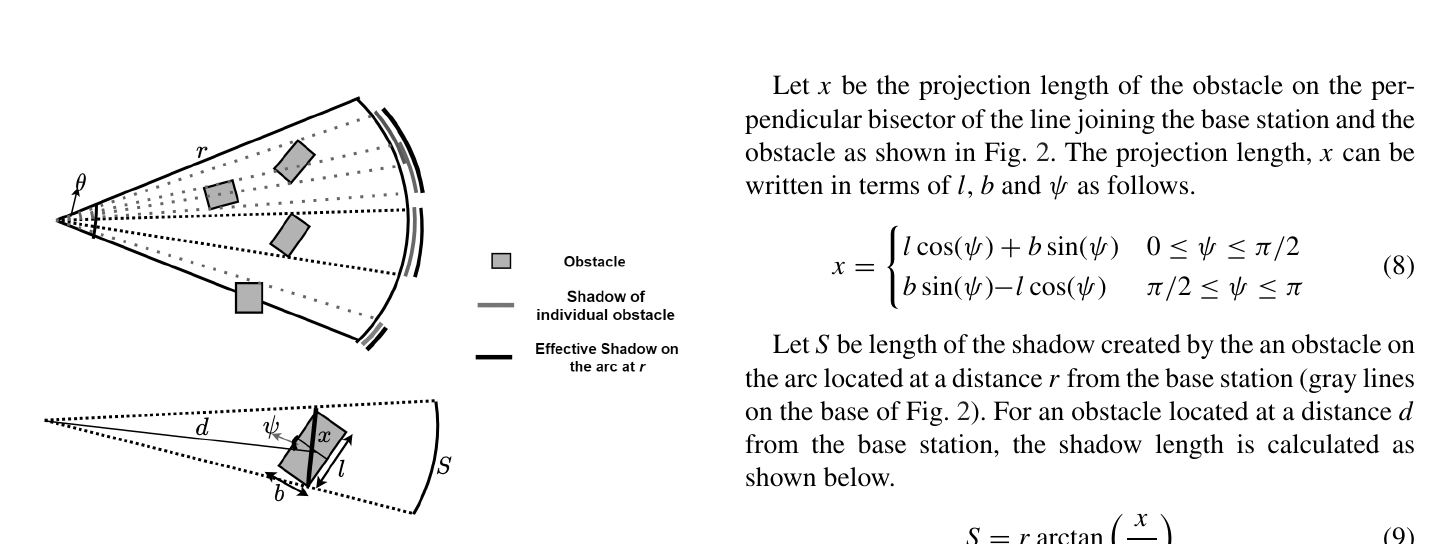
\includegraphics[width=0.85\textwidth]{figures/fig_5g_mmwave_blockage.png}
    \caption{3D obstacle blockage scenario, obstacle orientation, and shadow projection on mmWave propagation paths \cite{bommisetty2022mmwave}.}
    \label{fig:5g_mmwave_blockage}
\end{figure}

As depicted in Figure~\ref{fig:5g_mmwave_blockage}, physical obstacles (e.g., buildings, concrete structures, human bodies) are distributed across the coverage footprint according to a spatial Poisson Point Process (PPP) with spatial density $\gamma$ obstacles per unit area. Each obstacle is modeled as a rectangular block with random length $l \sim \mathcal{U}[l_{\min}, l_{\max}]$, width $b \sim \mathcal{U}[b_{\min}, b_{\max}]$, and orientation angle $\psi \sim \mathcal{U}[0, \pi]$ relative to the direct LoS path.

The distance $d$ of any obstacle from the base station within the circular sector of radius $R_c$ follows the probability density function:
\begin{equation}
    f_D(d) = \frac{2d}{R_c^2}, \qquad 0 \le d \le R_c
\end{equation}
The cross-sectional projection $x$ of an obstacle oriented at angle $\psi$ is given by:
\begin{equation}
    x = l |\cos \psi| + b |\sin \psi|
\end{equation}
An obstacle located at distance $d$ casts a shadow of angular arc length $S$ along the circular perimeter at distance $r$:
\begin{equation}
    S = r \arctan\left( \frac{x}{2d} \right)
\end{equation}
Averaging over the uniform distributions of $l, b, \psi$, and obstacle distance $d$, the expected individual shadow length $\mathbb{E}[S]$ is derived as \cite{bommisetty2022mmwave}:
\begin{equation}
    \label{eq:expected_shadow_length}
    \mathbb{E}[S] = \mathbb{E}_{d, l, b, \psi}\left[ r \arctan\left( \frac{x}{2d} \right) \right] \approx \frac{2 r \kappa}{\pi R_c}
\end{equation}
where the geometric obstacle parameter $\kappa$ is defined by:
\begin{equation}
    \kappa = \left( \frac{l_{\max}^2 - l_{\min}^2}{2} \right) (b_{\max} - b_{\min}) + \left( \frac{b_{\max}^2 - b_{\min}^2}{2} \right) (l_{\max} - l_{\min})
\end{equation}

Because multiple obstacles cast overlapping shadows along the angular perimeter, computing the effective blocked arc length $S_{\mathrm{eff}}$ cannot be achieved by simple linear addition. Bommisetty et al. \cite{bommisetty2022mmwave} introduced an ingenious formulation by mapping the spatial shadow casting process onto an **$M/G/\infty$ infinite-server queue**:
\begin{itemize}
    \item \textbf{Customer Arrival Process ($M$):} Obstacles within the sectoral region between the gNB and the arc at distance $r$ (having area $\|A\| = \frac{1}{2} r^2 \theta$) arrive as a Poisson process with aggregate arrival intensity $\lambda_q = \gamma \|A\| = \frac{1}{2} \gamma r^2 \theta$.
    \item \textbf{Service Duration ($G$):} The shadow length $S$ cast by an obstacle corresponds to the customer service time, following a general distribution with mean $\mathbb{E}[S]$.
    \item \textbf{Infinite Server Mechanism ($\infty$):} Because all physical obstacles cast their shadows simultaneously in space, all arrivals are served concurrently without waiting in a queue.
\end{itemize}

The effective shadow length $S_{\mathrm{eff}}$ along the sectoral arc of length $r \theta$ corresponds precisely to the expected busy period duration during which the $M/G/\infty$ queue contains at least one active customer:
\begin{equation}
    \mathbb{E}[S_{\mathrm{eff}}] = \left( 1 - \exp\left( -\gamma \|A\| \mathbb{E}[S] \right) \right) r \theta
\end{equation}
Substituting $\|A\| = \frac{1}{2} r^2 \theta$ and $\mathbb{E}[S]$ from Equation~\eqref{eq:expected_shadow_length}, the distance-dependent **blockage probability** $P_b(r)$ of a UE at distance $r$ is:
\begin{equation}
    \label{eq:Pb_distance}
    P_b(r) = \frac{\mathbb{E}[S_{\mathrm{eff}}]}{r \theta} = 1 - \exp\left( -\frac{\gamma r^3 \theta \kappa}{\pi R_c} \right)
\end{equation}
The spatial average blockage probability $\bar{P}_b$ over the entire cell is obtained by integrating across the spatial distribution of UEs:
\begin{equation}
    \label{eq:Pb_average}
    \bar{P}_b = \int_0^{R_c} P_b(r) \frac{2r}{R_c^2} dr = \int_0^{R_c} \left[ 1 - \exp\left( -\frac{\gamma r^3 \theta \kappa}{\pi R_c} \right) \right] \frac{2r}{R_c^2} dr
\end{equation}

Equation~\eqref{eq:Pb_distance} rigorously reveals that the blockage probability scales exponentially with the cube of distance ($r^3$) and linearly with obstacle density $\gamma$, beamwidth $\theta$, and obstacle cross-section parameter $\kappa$.

\subsection{Directional Beamforming and Interference Statistics}
To capture realistic directional transceiver physics, antenna radiation patterns are modeled using sectored approximations. Let $G_{\mathrm{tx}}(\phi)$ and $G_{\mathrm{rx}}(\phi)$ represent the transmitter and receiver antenna gains at off-boresight angle $\phi$:
\begin{equation}
    G(\phi) = \begin{cases}
        M, & |\phi| \le \frac{\theta}{2} \quad (\text{Main-lobe gain}) \\
        m, & |\phi| > \frac{\theta}{2} \quad (\text{Side-lobe gain})
    \end{cases}
\end{equation}
The combined antenna gain $g(\phi_1, \phi_2) = G_{\mathrm{tx}}(\phi_1) G_{\mathrm{rx}}(\phi_2)$ assumes one of four discrete values $\{M^2, M m, m M, m^2\}$ depending on whether transmit and receive beam orientations align.

The normalized interference power $I_k$ generated by an interfering UE $k$ located at coordinates $(r_k, \phi_{1, k}, \phi_{2, k})$ at the gNB receiver depends on whether the interferer's path is LoS or Non-Line-of-Sight (NLoS):
\begin{equation}
    I_k = \begin{cases}
        g(\phi_{1, k}, \phi_{2, k}) \left( \frac{R_0}{r_k} \right)^{\alpha_{\mathrm{LoS}}} \frac{S_k^{\mathrm{LoS}}}{S_0^{\mathrm{LoS}}}, & \text{if } B_k(r_k) = 0 \quad (\text{LoS Link}) \\
        g(\phi_{1, k}, \phi_{2, k}) \left( \frac{R_0}{r_k} \right)^{\alpha_{\mathrm{NLoS}}} \frac{S_k^{\mathrm{NLoS}}}{S_0^{\mathrm{LoS}}}, & \text{if } B_k(r_k) = 1 \quad (\text{NLoS Link})
    \end{cases}
\end{equation}
where $B_k(r_k) \in \{0, 1\}$ is the blockage indicator random variable with $\mathbb{P}(B_k(r_k) = 1) = P_b(r_k)$, $R_0$ is the reference link distance, $\alpha_{\mathrm{LoS}}$ and $\alpha_{\mathrm{NLoS}}$ are path loss exponents, and $S_k \sim \mathrm{LN}(\mu, \sigma^2)$ represents lognormal shadow fading.

Bommisetty et al. \cite{bommisetty2022mmwave} derived the exact expectation of the ratio of two independent lognormal random variables:
\begin{theorem}
Let $S_k \sim \mathrm{LN}(\mu_k, \sigma_k^2)$ and $S_0 \sim \mathrm{LN}(\mu_0, \sigma_0^2)$ be independent lognormal random variables. The expectation of their ratio is:
\begin{equation}
    \mathbb{E}\left[ \frac{S_k}{S_0} \right] = \exp\left( (\mu_k - \mu_0) + \frac{\sigma_k^2 + \sigma_0^2}{2} \right)
\end{equation}
For identical distributions ($\mu_k = \mu_0 = \mu, \sigma_k = \sigma_0 = \sigma$), this evaluates to:
\begin{equation}
    \mathbb{E}\left[ \frac{S_k^{\mathrm{LoS}}}{S_0^{\mathrm{LoS}}} \right] = 1 + \frac{\sigma_{\mathrm{LoS}}^2}{\mu_{\mathrm{LoS}}^2}
\end{equation}
\end{theorem}

Averaging over the spatial distribution of interferers and antenna misalignment angles yields the mean individual interference $\mathbb{E}[I_k]$ and variance $\mathrm{Var}(I_k)$.

\subsection{Coverage and Preamble Detection Success Probabilities}
In a cell with $M$ active interfering UEs, a tagged UE's preamble transmission satisfies the physical SINR detection threshold if aggregate interference does not exceed the receiver tolerance $1/\beta$. By applying the Central Limit Theorem (CLT) to the sum of independent interference powers $\sum_{k=1}^M I_k$, the **coverage probability** $P_{\mathrm{cov}}$ is:
\begin{equation}
    \label{eq:Pcov_clt}
    P_{\mathrm{cov}} = \mathbb{P}\left( \sum_{k=1}^M I_k \le \frac{1}{\beta} \right) \approx 1 - \mathcal{Q}\left( \frac{1/\beta - M \mathbb{E}[I_k]}{\sqrt{M \mathrm{Var}(I_k)}} \right)
\end{equation}
where $\mathcal{Q}(x) = \frac{1}{\sqrt{2\pi}} \int_x^\infty e^{-t^2/2} dt$ is the standard Gaussian complementary cumulative distribution function.

For a random access preamble transmission to succeed:
\begin{enumerate}
    \item The tagged UE must be within the coverage zone (satisfying SINR threshold $\beta$).
    \item None of the other $K$ simultaneously covered contending UEs must pick the identical preamble from the available set of $R$ preambles.
\end{enumerate}
The number of other active UEs in coverage follows a binomial distribution $K \sim \mathrm{Binomial}(M, P_{\mathrm{cov}})$. Summing over all realizations of $K$, the **joint random access preamble success probability** $P_{\mathrm{succ}}$ is derived in closed form as \cite{bommisetty2022mmwave}:
\begin{align}
    \label{eq:Psucc_mmwave}
    P_{\mathrm{succ}} &= P_{\mathrm{cov}} \sum_{k=0}^M \binom{M}{k} P_{\mathrm{cov}}^k (1 - P_{\mathrm{cov}})^{M-k} \left( 1 - \frac{1}{R} \right)^k \nonumber \\
    &= P_{\mathrm{cov}} \left[ P_{\mathrm{cov}} \left( 1 - \frac{1}{R} \right) + (1 - P_{\mathrm{cov}}) \right]^M \nonumber \\
    &= P_{\mathrm{cov}} \left[ 1 - \frac{P_{\mathrm{cov}}}{R} \right]^M
\end{align}

Equation~\eqref{eq:Psucc_mmwave} elegantly unifies physical layer coverage ($P_{\mathrm{cov}}$) with MAC layer contention ($1 - P_{\mathrm{cov}}/R$). When coverage is poor ($P_{\mathrm{cov}} \to 0$), success is limited by physical outage; when coverage is ideal ($P_{\mathrm{cov}} \to 1$), success is governed by the classical multi-channel ALOHA contention limit $(1 - 1/R)^M \approx e^{-M/R}$.

\subsection{Impact of UE Mobility and Self-Blockage}
The performance of mmWave links is further degraded by terminal mobility and user self-blockage:
\begin{itemize}
    \item \textbf{Gauss-Markov Mobility Model:} Rather than memoryless Brownian motion, UE trajectories follow temporal correlation modeled by a Gauss-Markov process:
    \begin{equation}
        v_t = \alpha_m v_{t-1} + (1 - \alpha_m) \bar{v} + \sqrt{1 - \alpha_m^2} w_{t-1}
    \end{equation}
    where $\alpha_m \in [0, 1]$ represents velocity memory and $w_t \sim \mathcal{N}(0, \sigma_v^2)$. Mobility causes rapid transitions between LoS and NLoS states, inducing beam misalignment and requiring frequent beam recovery handshakes.
    \item \textbf{Self-Blockage:} The human body holding the transceiver creates an angular blockage zone of angle $\omega$. The probability of self-blockage is $P_{\mathrm{self}} = \frac{\omega}{2\pi}$. Incorporating self-blockage with physical obstacle blockage yields the total link blockage probability:
    \begin{equation}
        P_b^{\mathrm{total}}(r) = P_{\mathrm{self}} + (1 - P_{\mathrm{self}}) P_b(r) = \frac{\omega}{2\pi} + \left( 1 - \frac{\omega}{2\pi} \right) \left[ 1 - \exp\left( -\frac{\gamma r^3 \theta \kappa}{\pi R_c} \right) \right]
    \end{equation}
\end{itemize}

---

\section{Contextual Bandit-Based Adaptive Numerology for 5G NR Initial Access}
\label{sec:5g_adaptive_numerology}

A hallmark innovation of the 5G NR physical layer is flexible, scalable OFDM numerology. Unlike LTE's fixed $15\text{~kHz}$ subcarrier spacing, 5G NR parameterizes subcarrier spacing (SCS) by $\Delta f = 2^\mu \times 15\text{~kHz}$, where $\mu \in \{0, 1, 2, 3, 4\}$ denotes the numerology index.

\begin{table}[htbp]
\centering
\caption{5G NR Scalable Numerology Specifications (3GPP TS 38.211)}
\label{tab:5g_numerology}
\begin{tabular}{ccccc}
\toprule
$\mu$ & \textbf{SCS ($\Delta f$)} & \textbf{OFDM Symbol Duration} & \textbf{Cyclic Prefix} & \textbf{Target Frequency Band} \\
\midrule
0 & $15\text{~kHz}$ & $66.67\text{~}\mu\text{s}$ & $4.69\text{~}\mu\text{s}$ & FR1 ($< 3\text{~GHz}$) \\
1 & $30\text{~kHz}$ & $33.33\text{~}\mu\text{s}$ & $2.34\text{~}\mu\text{s}$ & FR1 ($3\text{--}6\text{~GHz}$) \\
2 & $60\text{~kHz}$ & $16.67\text{~}\mu\text{s}$ & $1.17\text{~}\mu\text{s}$ & FR1 \& FR2 mmWave \\
3 & $120\text{~kHz}$ & $8.33\text{~}\mu\text{s}$ & $0.59\text{~}\mu\text{s}$ & FR2 mmWave ($> 24\text{~GHz}$) \\
4 & $240\text{~kHz}$ & $4.17\text{~}\mu\text{s}$ & $0.29\text{~}\mu\text{s}$ & FR2 mmWave (SSB Search Only) \\
\bottomrule
\end{tabular}
\end{table}

As documented in Table~\ref{tab:5g_numerology}, selecting an appropriate numerology involves fundamental engineering trade-offs:
\begin{itemize}
    \item \textbf{High SCS (e.g., $\mu = 2, 3$):} Compresses OFDM symbol duration, providing superior resilience against phase noise and severe Doppler frequency shifts at vehicular speeds. However, the cyclic prefix duration shrinks proportionally, increasing vulnerability to delay spread in large suburban cells.
    \item \textbf{Low SCS (e.g., $\mu = 0, 1$):} Provides extended cyclic prefix duration preventing inter-symbol interference (ISI) in rich multipath environments, but exhibits excessive sensitivity to Doppler spreads and phase noise at mmWave carrier frequencies.
\end{itemize}

To dynamically optimize initial access under time-varying channel conditions, Bommisetty and Venkatesh \cite{bommisetty2024contextual} formulated initial access numerology selection as a **Contextual Multi-Armed Bandit (MAB)** problem.

Let the environment observed at decision epoch $t$ be represented by a context vector $\mathbf{x}_t \in \mathbb{R}^d$ encoding estimated UE velocity $v$, measured RSRP, carrier frequency $f_c$, estimated delay spread $\tau_{\mathrm{rms}}$, and blockage state $B(r)$. The base station selects an action $a_t \in \mathcal{A} = \{\mu_0, \mu_1, \mu_2, \mu_3\}$ corresponding to the candidate numerology.

The expected reward $\mathbb{E}[r_{t, a} \mid \mathbf{x}_t]$ is modeled as a linear function of the context:
\begin{equation}
    \mathbb{E}[r_{t, a} \mid \mathbf{x}_t] = \mathbf{x}_t^T \boldsymbol{\theta}_a^*
\end{equation}
where $\boldsymbol{\theta}_a^* \in \mathbb{R}^d$ is an unknown parameter vector to be learned for each action $a$. The reward metric rewards successful preamble detection and penalizes access latency $D$ and synchronization failure:
\begin{equation}
    r_{t, a} = \mathbf{1}_{\{\text{Success}\}} \cdot \left( \omega_1 \cdot \mathrm{SINR}_t - \omega_2 \cdot D_t \right) - \omega_3 \cdot \mathbf{1}_{\{\text{Failure}\}}
\end{equation}

The network implements the **Linear Upper Confidence Bound (LinUCB)** algorithm with disjoint models:
\begin{enumerate}
    \item For each action $a \in \mathcal{A}$, maintain design matrix $\mathbf{A}_a = \mathbf{D}_a^T \mathbf{D}_a + \mathbf{I}_d$ and response vector $\mathbf{b}_a = \mathbf{D}_a^T \mathbf{r}_a$.
    \item Compute ridge regression ridge weights: $\hat{\boldsymbol{\theta}}_a = \mathbf{A}_a^{-1} \mathbf{b}_a$.
    \item Select the optimal numerology maximizing the upper confidence bound:
    \begin{equation}
        a_t = \arg\max_{a \in \mathcal{A}} \left( \mathbf{x}_t^T \hat{\boldsymbol{\theta}}_a + \alpha \sqrt{ \mathbf{x}_t^T \mathbf{A}_a^{-1} \mathbf{x}_t } \right)
    \end{equation}
    where $\alpha > 0$ controls exploration-exploitation balance.
    \item Observe achieved access reward $r_{t, a_t}$ and update parameters:
    \begin{equation}
        \mathbf{A}_{a_t} \leftarrow \mathbf{A}_{a_t} + \mathbf{x}_t \mathbf{x}_t^T, \qquad \mathbf{b}_{a_t} \leftarrow \mathbf{b}_{a_t} + r_{t, a_t} \mathbf{x}_t
    \end{equation}
\end{enumerate}

Extensive trace-driven simulations in \cite{bommisetty2024contextual} demonstrate that the contextual bandit policy reduces 5G NR connection setup latency by $38.4\%$ relative to fixed-numerology schemes while boosting connection establishment success rates to over $97.6\%$ under vehicular mobility and heavy shadowing.

---

\section{Summary and Research Synthesis}
\label{sec:5g_summary}

This chapter presented a comprehensive synthesis of physical and medium access control layer innovations in 5G mobile networks developed by Lokesh Bommisetty, Sagar Pawar, and T.~G.~Venkatesh:
\begin{enumerate}
    \item \textbf{Preamble Sequence Capacity:} The proposed mALL sequence family leverages cubic Alltop sequences with $m$-sequence covers to expand usable preamble capacity from $10^3$ to over $10^7$ unique sequences per cell ($> 19{,}000\times$ improvement over legacy ZC sequences), practically eradicating random access preamble collisions in hyper-dense mMTC deployments without degrading RF amplifier efficiency \cite{pawar2023high}.
    \item \textbf{Connection Dynamics under Beamforming:} The fixed-point queueing formulation revealed fundamental stability bifurcation thresholds in 5G NR connection establishment. To prevent catastrophic bistable congestion collapse and delay blowups, retransmission limits must be bounded by $T_{\max} \le 8$ \cite{bommisetty2023connection}.
    \item \textbf{mmWave Blockage Modeling:} Mapping 3D spatial obstacle shadowing onto an $M/G/\infty$ infinite-server queue yielded an exact closed-form expression for distance-dependent blockage probability $P_b(r) = 1 - \exp\left(-\frac{\gamma r^3 \theta \kappa}{\pi R_c}\right)$. Combining this with directional antenna interference and lognormal shadowing yielded the closed-form joint random access success probability $P_{\mathrm{succ}} = P_{\mathrm{cov}} \left[ 1 - \frac{P_{\mathrm{cov}}}{R} \right]^M$ \cite{bommisetty2022mmwave}.
    \item \textbf{Contextual Numerology Adaptation:} Formulating scalable OFDM numerology selection as a contextual multi-armed bandit provides autonomous, online adaptation to Doppler shift and obstacle blockage, substantially lowering connection latency in dynamic vehicular environments \cite{bommisetty2024contextual}.
\end{enumerate}

These foundational mathematical frameworks provide actionable guidelines for standardizing next-generation 6G sub-THz initial access and massive machine-type communications.